% !TEX root = task4.tex
% -----------------------------------------------------------------
% Filename  :	task4_stateMachine_writeAllocatePolicy.tex
% Author    :	Carsten Hoppe
% Date		:	28. Januar 2017
% Reference	:	http://www.texample.net/tikz/examples/state-machine/
%				https://martin-thoma.com/how-to-draw-a-finite-state-machine/
% -----------------------------------------------------------------
%\tikzstyle{every state}=[fill=mycolor,text=white,minimum width=2cm]

\begin{tikzpicture}[->,>=stealth',shorten >=1pt,auto,
                    semithick,/tikz/initial text=Reset]
    
	% ------------------------------------------------------------------------------
    % Definition of tikz styles.       
	% ------------------------------------------------------------------------------
	\tikzstyle{vertex}=[state,fill=mycolor,text=white,minimum width=1cm]
	\tikzstyle{edge}  =[draw,thick,->]
	
	% ------------------------------------------------------------------------------
	% Definition of nodes.
	% ------------------------------------------------------------------------------
	[align=center,xscale=1,node distance=2cm and 4cm]
	\node[initial,vertex]	(A)                    		{\tiny $IDLE$};
  	\node[vertex]         	(B) [below left=4cm of A] 	{\tiny $CW$};
  	\node[vertex]         	(C) [below=4cm of B] 		{\tiny $CMW$};
  	\node[vertex]         	(D) [below left=4cm of C] 	{\tiny $WBW$};
  	\node[vertex]         	(E) [below right=4cm of D] 	{\tiny $WCW$};
  	\node[vertex]		    (F) [below right=4cm of A] 	{\tiny $CR$};
  	\node[vertex]		    (G) [below =4cm of F] 		{\tiny $CMR$};
  	\node[vertex]		    (H) [below right=4cm of G] 	{\tiny $WBR$};
  	\node[vertex]		    (I) [below left=4cm of H] 	{\tiny $WCR$};

	% ------------------------------------------------------------------------------
	% Definition of paths.
	% ------------------------------------------------------------------------------
	\path (A) [edge, midway, above, sloped] edge node {CPU Write Request/-} (B)
		  (B) [edge, midway, above, sloped] edge node {Cache Miss/Stall Processor} (C)
		  (C) [edge, midway, above, sloped] edge node {Replaced Block Is Dirty/Write Replaced Block To Memory} (D)
		  (D) edge node [midway, above, sloped] {0,1,L} (E)
		  (E) [edge, midway, above, sloped] edge node {readyMEM=1/Write Data Into Cache, Set Dirty Bit (Modified) Bit} (A);
		  
	\path (A) [edge, midway, above, sloped] edge node {CPU Read Request/-} (F)
		  (F) [edge, midway, above, sloped] edge node {Cache Miss/Stally Processor} (G)
		  (G) [edge, midway, above, sloped] edge node {Replaced Block Is Dirty/Write Replaced Block To Memory} (H)
		  (H) [edge, midway, above, sloped] edge node {0,1,L} (I)
		  (I) [edge, midway, above, sloped] edge node {readyMEM=1/Read Data Into CPU} (A);

		
\end{tikzpicture}


\begin{table}
\caption{Overview - FSM States}
\label{tab:tableFSM}
\begin{tabular}{llll}
\hline %\toprule
Abbreviation & Name & CPU Request Mode & Description \\
\hline %\midrule
IDLE 	& -					& - 			& - \\
CW		& COMPARE WRITE		& Write Request & - \\
CMW		& CACHE MISS WRITE	& Write Request & - \\
WBW		& WRITE BACK WRITE	& Write Request & - \\
WCW		& WRITE CACHE WRITE	& Write Request & - \\
CR		& COMPARE READ		& Read Request 	& - \\
CMR		& CACHE MISS READ	& Read Request 	& - \\
WBR		& WRITE BACK READ	& Read Request 	& - \\
WCR		& WRITE CACHE READ	& Read Request 	& - \\
\hline %\bottomrule
\end{tabular} 
\end{table}


\begin{figure}
	\centering
	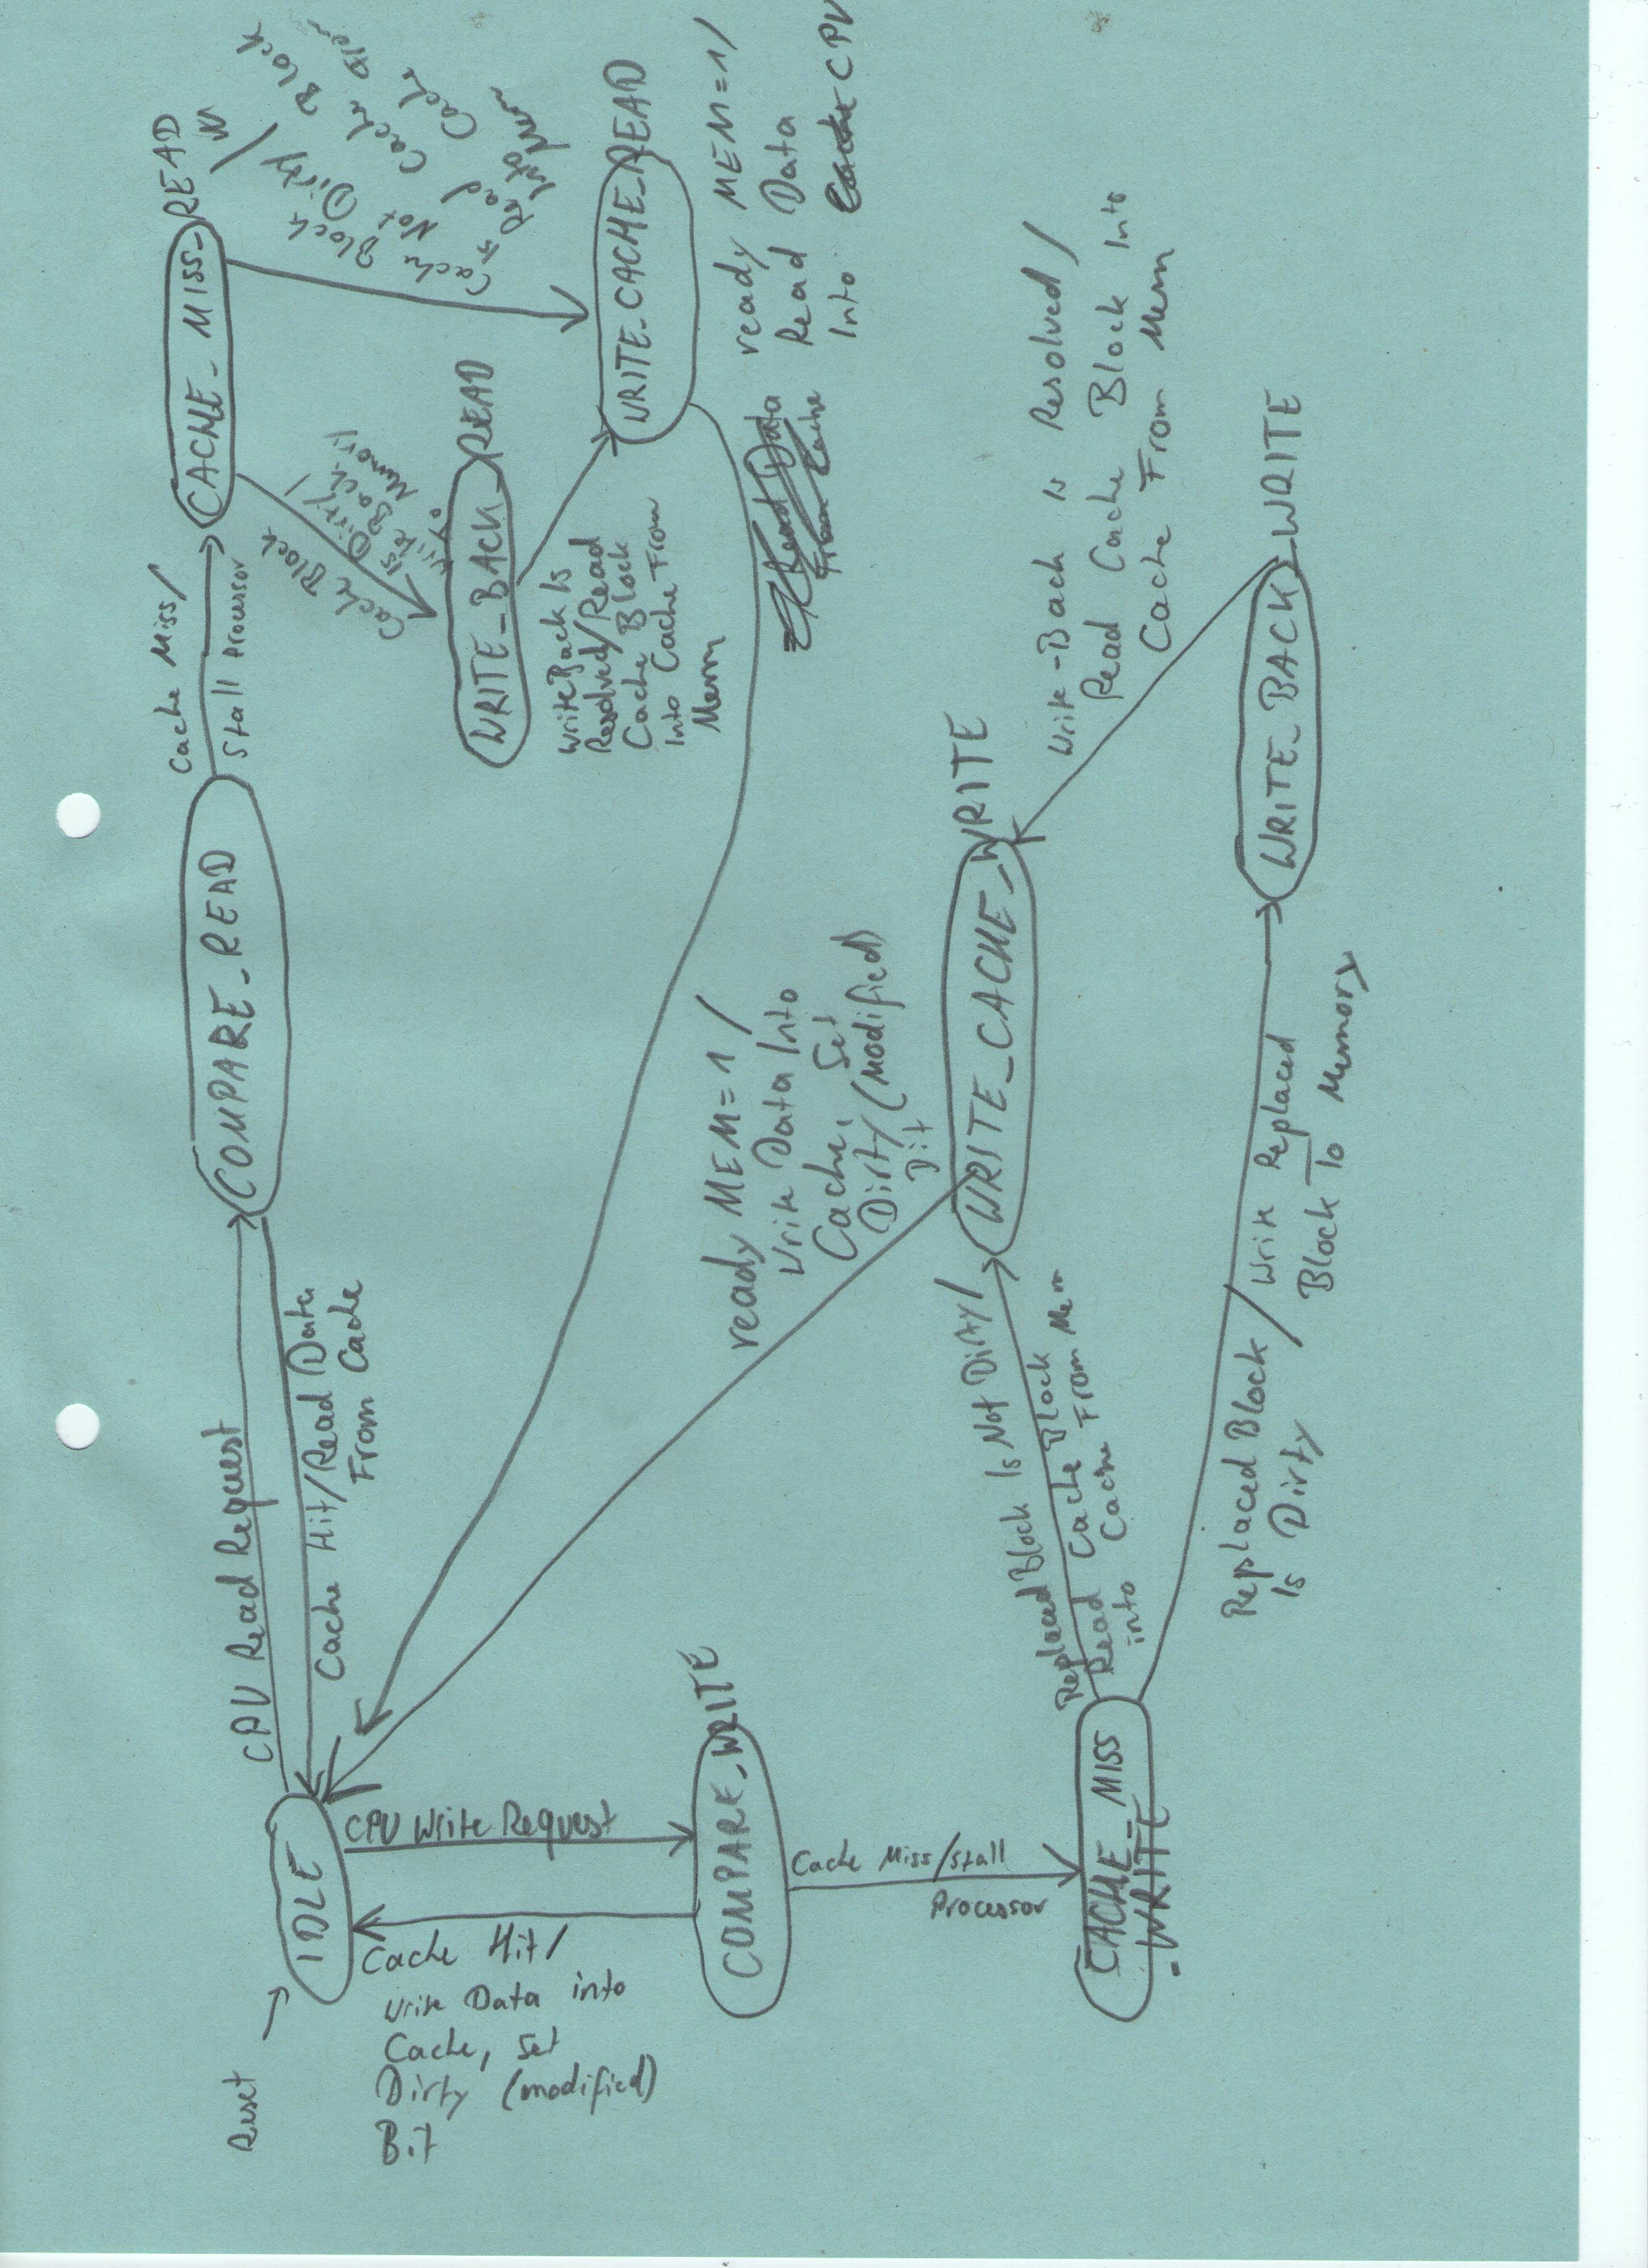
\includegraphics[scale=.8]{pictures/sketch_mealyAutomata}
	\caption{Sketch of Mealy Automata - Cache Controller}
	\label{fig:sketchMealyAutomata}
\end{figure}
